\chapter{Synchrone Machines}
Synchrone machines zijn machines die werken op een \textbf{constante snelheid}, de
synchrone snelheid.
Ze werken op AC en kunnen gebruikt worden als motor en generator.
Het is de rotor dat wordt meegesleurd door het draaiveld van de stator (\textbf{anker},
let dus op want hier is de stator het anker, niet de rotor!!).
De opbouw van de stator die we eerder zagen is hetzelfde hier, en het principe met het
draaiveld dus ook, het is de rotor die we in de stator brengen dat kan verschillen qua
opbouw.

\section{Rotor}
Voor de opbouw van de rotor kunnen we met \textbf{permanente magneten} werken of met
\textbf{DC-windingen}, de volgende figuur toont hoe de statorgleuven gevuld zijn met koper
en een rotor met permanente magneten daarin is gebracht, we zien dat de permanente
magneten hier ook tussen ijzergleuven zitten op de rotor.

\begin{figure}[H]
  \centering
  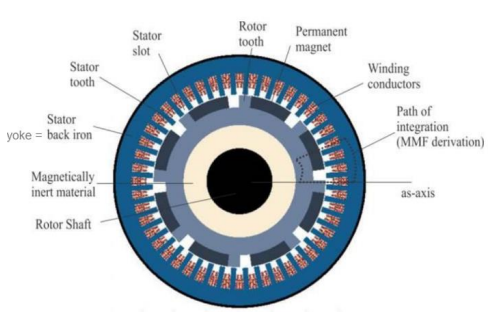
\includegraphics[width=0.6\textwidth]{assets/permanentemagneterotorinstator.png}
  \caption{Permanentemagneten rotor in stator}
  \label{fig:permanentemagneterotorinstator.png}
 \end{figure}

De rotor kan echter ook een \textbf{gladde rotor} zijn of een rotor met
\textbf{uitspringende polen}, met een gladde rotor bedoelen we hier wel 'magnetisch glad'
(weinig reluctantie), mechanisch heeft die gleuven met magneten.
Uitspringende polen is vooral bij kleine machines en glad bij grote.

Hier zien we een figuur van permanente magneten en een rotor met DC-windingen, het veld
word extern geëxciteerd met een veldstroom If:

\begin{figure}[H]
  \centering
  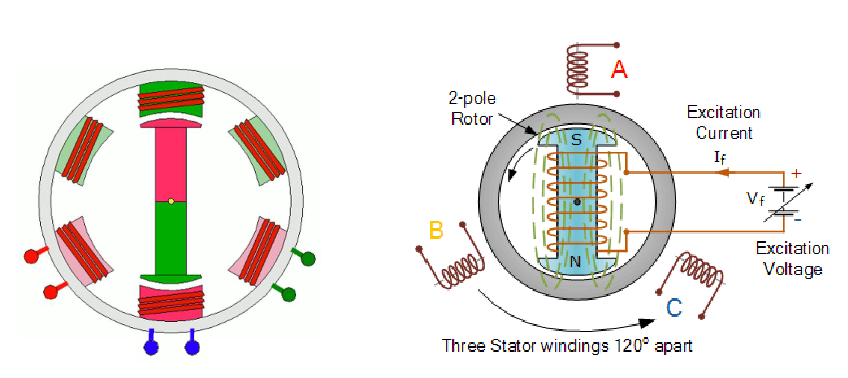
\includegraphics[width=0.6\textwidth]{assets/PMvsDCwindinge.png}
  \caption{PM vs DC windingen}
  \label{fig:PMvsDCwindinge.png}
 \end{figure}

\section{Stator en rotor magnetisch veld}
Eigelijk zijn er 2 draaivelden nu, we hebben dus het draaiveld van de stator dat opgewekt
wordt door de 3AC dat we eerder bespraken maar we hebben ook een draaiveld in de rotor dat
opgewekt wordt door de DC-windingen, maar let goed op, dit is een \textbf{constant} veld,
het draait dus niet mee met de rotor.
Het is dus de rotor die meegesleurd wordt door het draaiveld van de stator wat het dus
doet lijken dat het veld van de rotor draait als je langs buiten kijkt of als je kijkt
vanuit de stator zelf (want die staat stil).

Dus we hebben \textbf{$B_s$} dat het draaiveld van de stator is met elektrische pulsatie
$\omega_s$ opgewekt door de 3AC en we hebben \textbf{$B_R$} dat het veld van de rotor is
opgewekt door de DC-veldstroom $i_f$ in de rotor dat vast is tegenover de rotor maar
mechanisch mee draait met de rotor.
Deze 2 moeten dus dezelfde snelheid hebben want het statorveld sleurt de rotor mee, en
hiermee wordt dus dat koppel gegenereerd met:
\begin{align*}
  \vv{T} = k \cdot \vv{B}_s \times \vv{B}_R
\end{align*}
k is trouwens een constante

Dan hebben we ook nog het \textbf{mutueel magnetisch veld} dat ontstaat door de interactie
van de 2 velden, het is waar $B_s$ en $B_R$ samen komen en optellen tot één totaal veld:
\begin{align*}
  \vv{B}_{mut} = \vv{B}_s + \vv{B}_R
\end{align*}
De formule voor het koppel kan ook geschreven worden als:
\begin{align*}
  \vv{T} = k \cdot \vv{B}_{mut} \times \vv{B}_R
\end{align*}
Dit is exact hetzelfde als hierboven, als je dit uitwerkt kom je op dezelfde formule want
dit werkt met kruisproducten, als je dit raar vind, vraag het aan AI.

\begin{figure}[H]
  \centering
  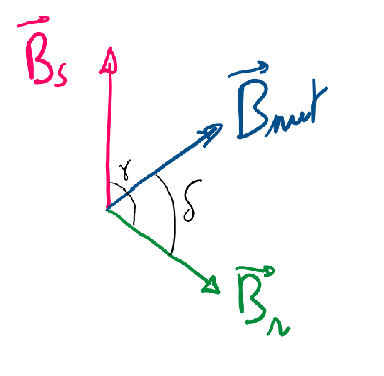
\includegraphics[width=0.4\textwidth]{assets/vectorschemaBsenBr.png}
  \caption{Vector schema van $B_s$ en $B_R$}
  \label{fig:vectorschemaBsenBr.png}
 \end{figure}

In de figuur hierboven zien we hoe $B_s$ en $B_R$ samen een mutueel veld vormen vectorieel
weergegeven.
Als je de vector formules van hierboven uitwerkt heb je per definitie altijd de hoek
tussen je 2 vectoren nodig want
$|\vv{A} \times \vv{B}| = |\vv{A}| \cdot |\vv{B}| \cdot \sin(\theta)$, en dit is dus de
hoek tussen de 2 vectoren.
De 2 hoeken voor deze vectoren zijn weergegeven op de figuur (met $\delta$ de koppelhoek,
die we zometeen bespreken).

\begin{figure}[H]
  \centering
  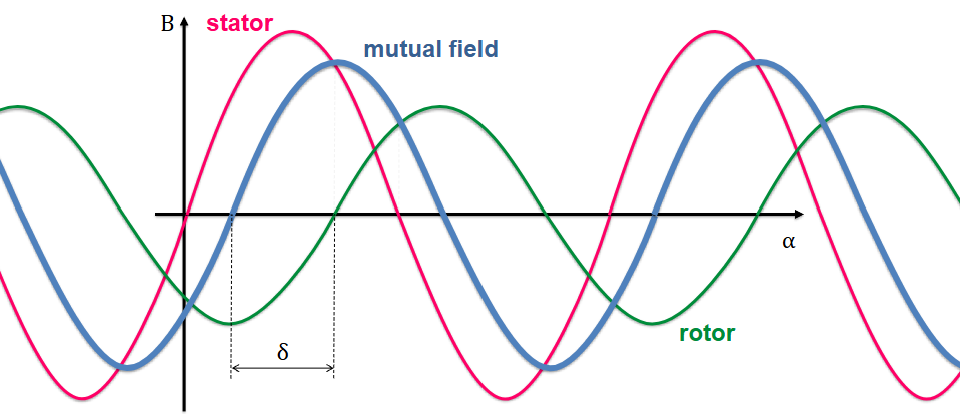
\includegraphics[width=0.5\textwidth]{assets/sinusoidaleweergavemutueelveld.png}
  \caption{Sinusoidale weergave van het mutueel veld}
  \label{fig:sinusoidaleweergavemutueelveld.png}
 \end{figure}

In de figuur hierboven zien we hoe het mutueel veld er uitziet in een sinusvorm, hier is
de koppelhoek een faseverschuiving eigelijk.
Dit is echter wel minder simpel weer te geven dan vectorieel dus vanaf nu doen we het
gewoon vectorieel.

\section{Koppelhoek/Lasthoek}
De koppelhoek (ook wel lasthoek genoemd) is de hoek tussen het statorveld en het
rotorveld, het wordt niet echt deftig vermeld op de slides of in de les maar in principe
is het een elektrische hoek dat ook met het poolpaartal naar een mechanische hoek omgezet
kan worden, echter werkt de proff in de slides met voorbeelden waar de machines 2 polen
hebben en dus een poolpaartal van 1, daarom is het niet zo duidelijk want dan zijn die
gewoon gelijk aan elkaar.
Zoals we weten uit de vorige formules bepaalt deze hoek eigelijk het koppel dat de machine
kan leveren met $T = k \cdot B_{mut} \cdot B_R \cdot \sin(\delta)$, op de volgende figuur
zien we hoe het koppel wordt ontwikkeld voor elke toepassing van de synchrone machine:

\begin{figure}[H]
  \centering
  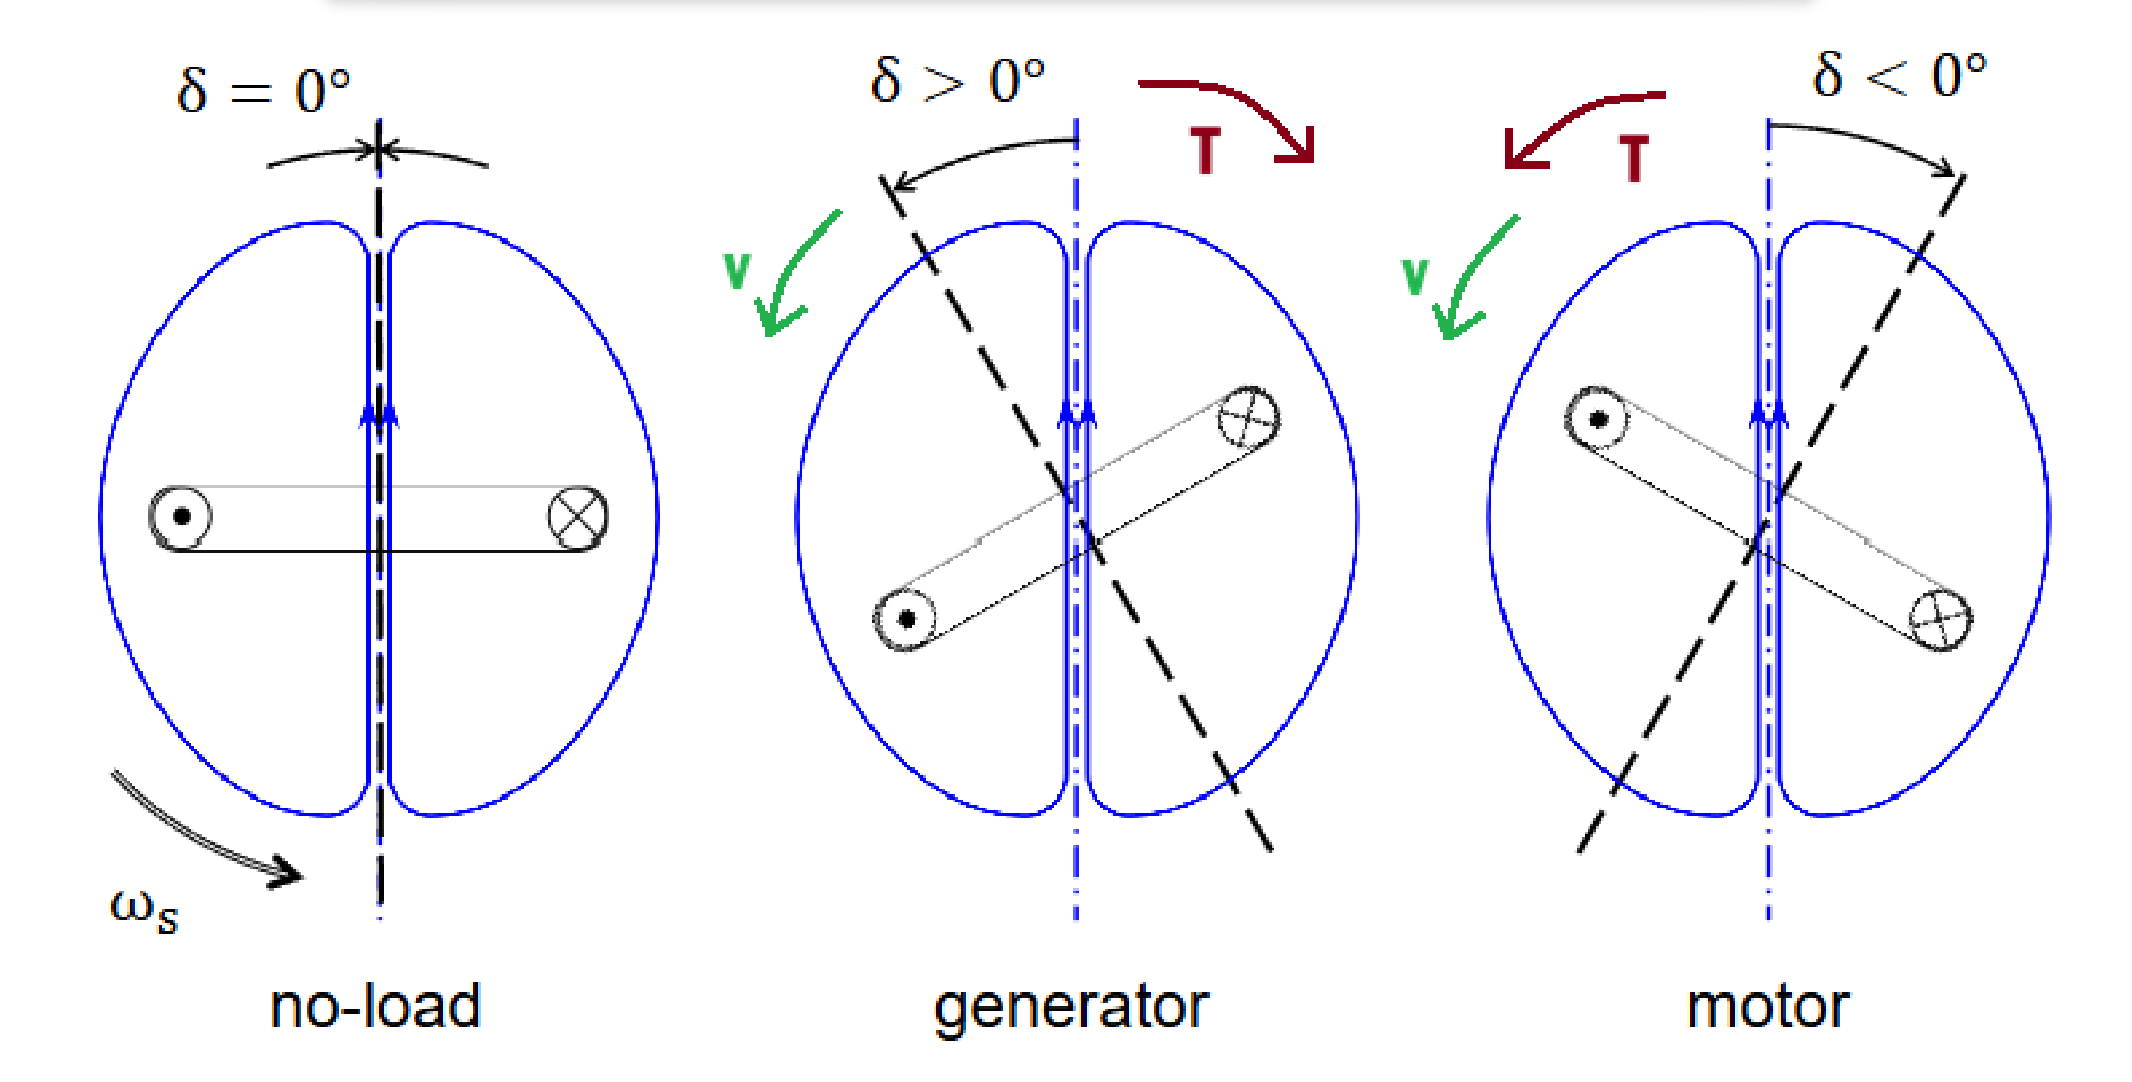
\includegraphics[width=0.6\textwidth]{assets/lasthoeknullastgeneratormotorsynchronemachine.png}
  \caption{Lasthoek bij nullast, generator en motor van een synchrone machine}
  \label{fig:lasthoeknullastgeneratormotorsynchronemachine.png}
 \end{figure}

\subsubsection{Nullast}
Dit is niet hetzelfde als stil staan, er is hier gewoon geen last (dus \textbf{geen
koppel, $T = 0$}).
De \textbf{motor draait wel op volle snelheid} daardoor en de stator trekt de rotor dus
niet mee, er is dus een \textbf{koppelhoek van 0°}.

\subsubsection{Generator}
Hier ijlt de rotor voor op het mutueel veld, hierdoor wordt er een koppel ontwikkeld dat
de rotor tegenhoudt, eigelijk tegenin de beweging van de rotor in, \textbf{de rotor trekt
dus het magnetisch veld mee}, het \textbf{koppel is tegengesteld aan de lasthoek} want het
wilt het terug brengen naar 0°.
Een referentie die we nemen om te zeggen of de hoekpositie van de lasthoek positief is, is
als hij in dezelfde richting is als de draaizin, wat hier het geval is, dus de
\textbf{lasthoek is positief.}

\subsubsection{Motor}
Hier wordt de rotor meegetrokken door het mutueel veld, dit wordt dus gecreëerd door de
3AC die het draaiveld vormen.
Het koppel werkt mee met de snelheid, doordat de rotor achterloopt is de \textbf{lasthoek}
in de andere richting als de beweging en dus \textbf{negatief}.
Hoe groter deze hoek tho (negatiever dan), hoe groter het koppel.

\section{Berekening van de geïnduceerde spanning}
We hebben dus onze 3AC machine met een stilstaande stator en een rotor die een constant
veld heeft en in de stator draait, dat constant veld dat door een DC-winding wordt
opgewekt gaat eigelijk langs de stator windingen passeren omdat de rotor draait en dus
daardoor een spanning induceren in de stator wikkelingen, deze gaan we nu berekenen hoe
groot die is.

\begin{figure}[H]
  \centering
  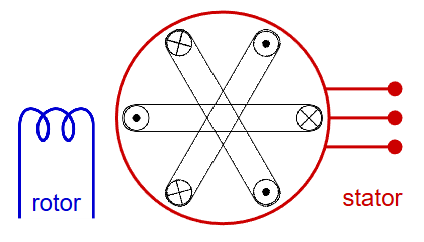
\includegraphics[width=0.6\textwidth]{assets/rotor_stator_doorsnede.png}
  \caption{Doorsnede van rotor en stator:
  de statorwikkeling bestaat uit 3 fasen, elk met hun eigen vaste positie $\theta$ rond de
  omtrek.}
  \label{fig:rotor_stator_doorsnede}
\end{figure}

\subsubsection{Flux gezien door een statorspoel}
Elke statorspoel zit op een \textit{vaste positie} $\theta_x$.
De mutuele flux die spoel $a$ (op positie $\theta_a$) ziet, is:
\begin{align*}
    \Phi_{mut,a} = \hat{\Phi} \cdot \cos(\omega_s t - p\theta_a)
\end{align*}
Omdat de drie fasespoelen elk op een andere positie ($\theta_a$, $\theta_b$, $\theta_c$,
telkens 120° elektrisch uit elkaar) rond de omtrek zitten, zien ze alle drie een
\textbf{andere} flux, vandaar dat elke fase zijn eigen (in tijd verschoven) spanning
krijgt.

\subsubsection{Geïnduceerde spanning via Faraday}
Met de wet van Faraday, $e = -N\dfrac{d\Phi}{dt}$, en
$\Phi_a(t) = \hat{\Phi}\cos(\omega_s t)$ voor spoel $a$ (referentiepositie $\theta_a=0$):
\begin{align*}
    e_a(t) = -N\frac{d\Phi_a}{dt} = N\hat{\Phi}\,\omega_s \sin(\omega_s t)
\end{align*}
Met de piekwaarde $\hat{E} = N\hat{\Phi}\,\omega_s$ (op tekenconventie na, afhankelijk van
de gekozen positieve richting) geeft dit voor de drie fasen:
\begin{align*}
    e_a(t) &= -\hat{E}\cdot\sin(\omega_s t) \\
    e_b(t) &= -\hat{E}\cdot\sin(\omega_s t - 120^\circ) \\
    e_c(t) &= -\hat{E}\cdot\sin(\omega_s t - 240^\circ)
\end{align*}

\subsubsection{Effectieve waarde}
De effectieve (RMS) waarde volgt weer uit de piekwaarde gedeeld door $\sqrt{2}$:
\begin{align*}
    \boxed{E = \sqrt{2}\pi N_c \hat{\Phi} f = k\hat{\Phi}\omega}
\end{align*}
Dit komt exact overeen met de formule uit de vorige sectie.
Merk ook op dat $E \sim I_f$ (evenredig met de rotor-veldstroom), net zoals bij de
magnetisatiecurve die we eerder zagen, maar geld dus ook niet heel de tijd.

\subsubsection{Aansluiting van de statorwikkeling}
De drie fasewikkelingen van de stator kunnen op twee manieren met elkaar verbonden worden:
in \textbf{ster (Y)} of in \textbf{driehoek ($\Delta$)}.
Deze keuze bepaalt de verhouding tussen lijn- en fasespanning/-stroom, en komt later
uitgebreider aan bod.

\subsubsection{Faseverhouding tussen flux, spanning en stroom}

\begin{figure}[H]
  \centering
  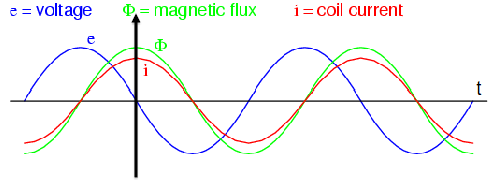
\includegraphics[width=0.7\textwidth]{assets/golfvormen_flux_spanning_stroom.png}
  \caption{Tijdsverloop van flux $\Phi$, geïnduceerde spanning $e$ en stroom $i$ in één
  fase.}
  \label{fig:golfvormen_flux_spanning_stroom}
\end{figure}

Uit de grafiek volgt de logische volgorde:
de flux $\Phi$ (cosinusvorm) bereikt zijn piek op $t=0$; de spanning $e=-N\,d\Phi/dt$
loopt daar $90^\circ$ op achter (nul op $t=0$, want de afgeleide van een piek is nul); En
die stroom i \textbf{is het model van de rotorstroom, het is de stroom die die groene flux
\textit{zou} maken als je het in de stator zou laten lopen, het is gewoon wat het zelfde
effect zou geven.
{\color{red}Dit is dus geen echte stroom!}}

\subsection{Magnetisatiecurve}
Dit hebben we eerder al wat gezien, maar komt terug rap voor op de slides.
Een andere benaming hier voor is trouwens de \textit{nullastkarakteristiek} of
\textit{open circuit karakteristiek}.

\begin{figure}[H]
  \centering
  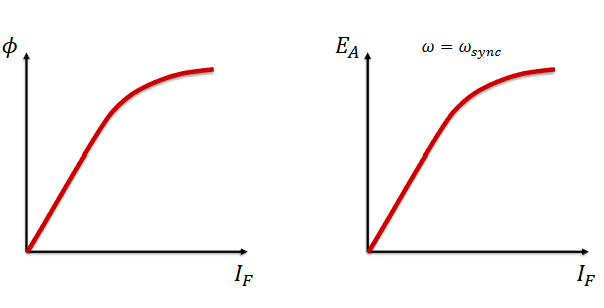
\includegraphics[width=0.6\textwidth]{assets/magnetscurves.png}
  \caption{Magnetisatiecurven}
  \label{fig:magnetscurves.png}
 \end{figure}

Bij de linkse curves zien we dat er even een lineair verband is tussen de hoeveelheid flux
en de veldstroom, maar dat dit na een bepaalde waarde niet meer zo is (saturatie) en dat
het veld maar een klein beetje meer toeneemt bij veel meer veldstroom.
De rechtse curve meten we door de spanning te meten bij een open klem (nullast) en op
constante volle snelheid van de motor (want $E = k\Phi\omega$).

Een belangrijk ding om op te merken is wel dat de inwendige spanning eigelijk toch niet
helemaal hetzelfde is als de klemspanning, dit komt door volgende verschillende effecten:

\begin{itemize}
   \item \textbf{Ankerreactie}:
   Dit is de belangrijkste, deze bespreken we zometeen uitgebreid
   \item \textbf{Zelfinductantie anker}:
   Dit is niet echt uitgelegd maar dit is gewoon de zelfinductantie van de
   statorwikkelingen, dit is een beetje zoals bij een DC-machine, als je een stroom door
   een spoel stuurt dan zal er een tegen EMK ontstaan dat de stroom tegenwerkt.
   Dit is dus ook zo bij de statorwikkelingen, als er een stroom doorheen gaat dan zal er
   een tegen EMK ontstaan dat de stroom tegenwerkt.
   \item \textbf{Ankerweerstand}: De weerstand van de statorwikkelingen
   \item \textbf{Uitspringende polen}:
   Dit is een mechanisch effect, dit is wel 'extra' dus is eigelijk niet belangrijk
\end{itemize}

\section{Ankerreactie}
Ankerreactie is simpelweg de stroom in de stator dat ook een veld veroorzaakt dat het
totale veld verstoort.
Hiervoor kijken we naar de fasediagrammen:

\begin{figure}[H]
  \centering
  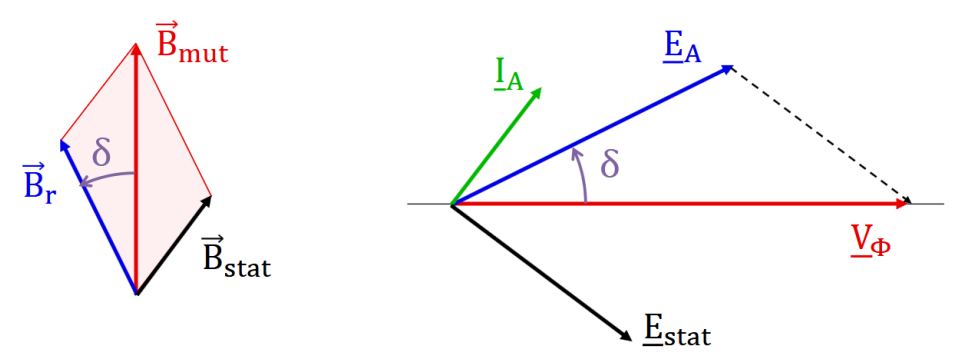
\includegraphics[width=0.6\textwidth]{assets/fasediagrammen.png}
  \caption{Fasediagram veld en Stroom/spanningen synchrone motor (Deze figuur is voor de
  Onderbekrachtigde Generator)}
  \label{fig:fasediagrammen.png}
 \end{figure}

We hebben dus het veld van de rotor $\vv{B}_R$ dat onder een bepaalde geometrische hoek in
de ruimte staat, het is dit veld dat de inwendige spanning $\underline{E}_A$ induceert in
de statorwikkelingen.
Als we dan onze motor gaan belasten dan zal er dus ook een stroom gaan lopen in de
statorwikkelingen, dit is de stroom $\underline{I}_A$, het is deze stroom dat dan ook een
magnetisch veld induceerd in de stator, dit is die ankerreactie eigelijk, het is
$\vv{B}_{Stat}$ dat samen met $\vv{B}_R$ een mutueel veld vormt $\vv{B}_{mut}$ dat de
rotor dus mee trekt.
Het veld van de stator $\vv{B}_{Stat}$ induceert dan ook nog $\underline{E}_{Stat}$ (de
spanningsval over de statorreactantie), deze bepaald eigelijk of de klemspanning
$\underline{V}_{\phi}$ groter of kleiner is dan de inwendige spanning $\underline{E}_A$.

\begin{warningbox}[Koppelhoek in deze figuur verschilt!]
    Let op want in de linkse figuur is de \textit{koppelhoek} bij die velden daar een
    \textbf{geometrische} hoek, maar in de rechtse figuur is dit de \textit{lasthoek}, dit
    is in het \textit{frequentiedomein} (tijd), het is een weergave voor
    \textbf{elektrische} grootheden dus!
\end{warningbox}

We kunnen de klemspanning dan ook als volgt schrijven:
\begin{align*}
    \underline{V}_{\phi} = \underline{E}_A + \underline{E}_{Stat}
\end{align*}
Hierbij is $\underline{E}_{Stat} = -j \cdot X \cdot \underline{I}_A$, dus de ankerreactie
wat te wijten is aan het feit dat de statorstroom het veld eigelijk verstoord.
Het is negatief omdat de stroom hier \textit{voor} ijlt op de spanning.

We hebben echter ook wel nog een zelfinductantie en een ankerweerstand, dus de volledige
vergelijking wordt dan:
\begin{equation*}
\underline{V}_{\phi} = \underline{E}_A
- \underbrace{\textcolor{blue}{j \cdot X \cdot \underline{I}_A}}_{\textcolor{blue}{\text{ankerreactie}}}
- \underbrace{\textcolor{red}{j \cdot X_A \cdot \underline{I}_A}}_{\textcolor{red}{\text{zelfinductantie}}}
- \underbrace{\textcolor{teal}{\underline{I}_A \cdot R}}_{\textcolor{teal}{\text{ankerweerstand}}}
\end{equation*}
Hierbij is die zelfinductantie eigelijk de invloed van \textbf{de stator OP DE STATOR}
zonder dat zelfs die rotor invloed heeft, het is gewoon lekflux eigelijk.
$X_A$ is de impedantie van de ankerreactie terwijl X de zelfinductantie is van het anker,
we gaan deze 2 samen nemen als $X_S$ zodat we het volgende krijgen:
\begin{align*}
    \underline{V}_{\phi} = \underline{E}_A - j \cdot X_S \cdot \underline{I}_A - \underline{I}_A \cdot R
\end{align*}
In ons equivalent model gaan we de ankerweerstand wel verwaarlozen, we gaan dus
idealiseren.
Dit maakt het dat we geen rendement kunnen bepalen, op het examen verwaarlozen we dit ook
maar kan ze het wel als theorievraag vragen wat het effect daarvan is.
We hebben dus:
\begin{align*}
    \underline{V}_{\phi} = \underline{E}_A - j \cdot X_S \cdot \underline{I}_A \\
    \rightarrow \underline{V}_{\phi} = j \cdot X_r \cdot \underline{I}_r - j \cdot X_S \cdot \underline{I}_A
\end{align*}
Hierboven is $E_A$ uitgeschreven als het model van het magnetisch effect van de rotor op
de stator met die rotorstroom $I_r$ dat eigelijk niet bestaat en de AC stroom zou zijn dat
het zelfde veld opwekt.

\newpage

\section{Equivalent schema}
In de volgende figuur zien we het equivalent circuit/model met een generatorreferentie:

\begin{figure}[H]
  \centering
  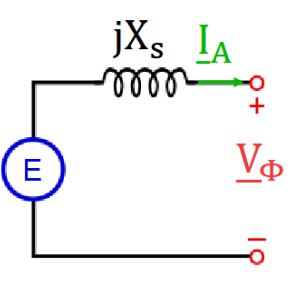
\includegraphics[width=0.3\textwidth]{assets/equivgenerref.png}
  \caption{Equivalent schema van een synchrone machine met generatorreferentie}
  \label{fig:equivgenerref.png}
 \end{figure}

De volgende figuur is dit dan voor een motorreferentie:

\begin{figure}[H]
  \centering
  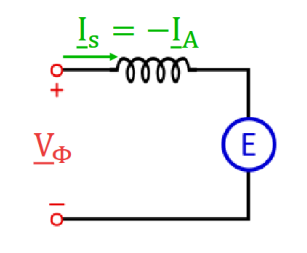
\includegraphics[width=0.3\textwidth]{assets/equimotorref.png}
  \caption{Equivalent schema van een synchrone machine met motorreferentie}
  \label{fig:equimotorref.png}
 \end{figure}

\subsection{Soorten metingen}
Er zijn een aantal proeven die we kunnen doen om de parameters te bepalen uit de formule
die we zojuist zagen, het gaat hier dan vooral om $E_A$ en $X_S$.

\subsubsection{Nullastproef}
Hierbij gaan we de rotor aandrijven tot de nominale (synchrone) snelheid en het veld
bekrachtigen met een aparte DC-bron en een regelbare weerstand die $I_f$ regelt.
De statorklemmen laten we open zodat $I_A = 0$ en dus de formule herleid naar:
\begin{align*}
    \underline{V}_{\phi} = \underline{E}_A
\end{align*}
De klemspanning kunnen we meten dus we hebben dan $E_A$ voor die specifieke $I_f$, dit
doen we voor verschillende veldstromen (stap verhogen steeds) om zo de volgende O.C.C.
kromme op te bouwen (O.C.C.
= Open Circuit Characteristic):

\begin{figure}[H]
  \centering
  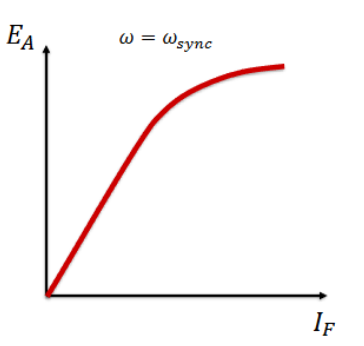
\includegraphics[width=0.3\textwidth]{assets/OCCcurve.png}
  \caption{O.C.C.}
  \label{fig:OCCcurve.png}
 \end{figure}

\begin{warningbox}[Hysteresis]
    Bij het verhogen van die stappen mag je NOOIT verlagen (terugdraaien) want je hebt
    hier hysteresis, ook zie je op het einde van de curve dat deze afbuigt, dit is
    verzadiging.
\end{warningbox}

\subsubsection{Kortsluitproef}
Dit heeft dezelfde opstelling, rotor tot nominale snelheid en veld bekrachtigen met aparte
DC bron maar nu gaan we de statorklemmen kortsluiten zodat $V_{\phi} = 0$ en dus de
formule herleid naar:
\begin{align*}
    0 = \underline{E}_A - j \cdot X_S \cdot \underline{I}_A \\
    \rightarrow j \cdot X_S \cdot \underline{I}_A = \underline{E}_A
\end{align*}
Zo meet je eigelijk $I_A$ ( = $I_{SC}$) voor verschillende veldstromen.
En omdat de kortsluitstroom via ankerreactie het netveld sterk demagnetiseert, blijft de
curve hier in het lineaire (onverzadigde) gebied, hoe groot $I_f$ ook is.

\begin{figure}[H]
  \centering
  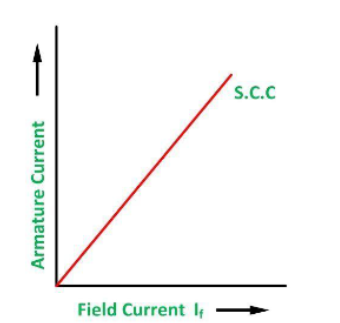
\includegraphics[width=0.3\textwidth]{assets/SCCcurve.png}
  \caption{S.C.C.}
  \label{fig:SCCcurve.png}
 \end{figure}

\subsubsection{Bepaling van de parameters}
Kies nu een veldstroom $I_f$ in de O.C.C.
en lees de corresponderende $E_A$ af.
Kies dezelfde $I_f$ in de S.C.C.
en lees de corresponderende $I_{SC}$ af.
Zo kan je dan $X_S$ berekenen met:
\begin{align*}
    X_S = \frac{E_A}{I_{SC}}
\end{align*}

\section{Fasediagrammen}
Via het equivalent circuit gaan we dus ook fasediagrammen kunnen opstellen, dit zijn
grafische weergaven van de grootheden in het complex vlak.
We hebben voor de synchrone machine een motorreferentie en een generatorreferentie, deze
verschillen dus.
Ook kunnen ze verschillen in over en onderbekrachtiging, dit is afhankelijk van de
veldstroom $I_f$ en de statorstroom $I_A$.
In de volgende figuren zien we de fasediagrammen voor een generator en een motor, beide
onder en overbekrachtigd:

\begin{figure}[H]
  \centering
  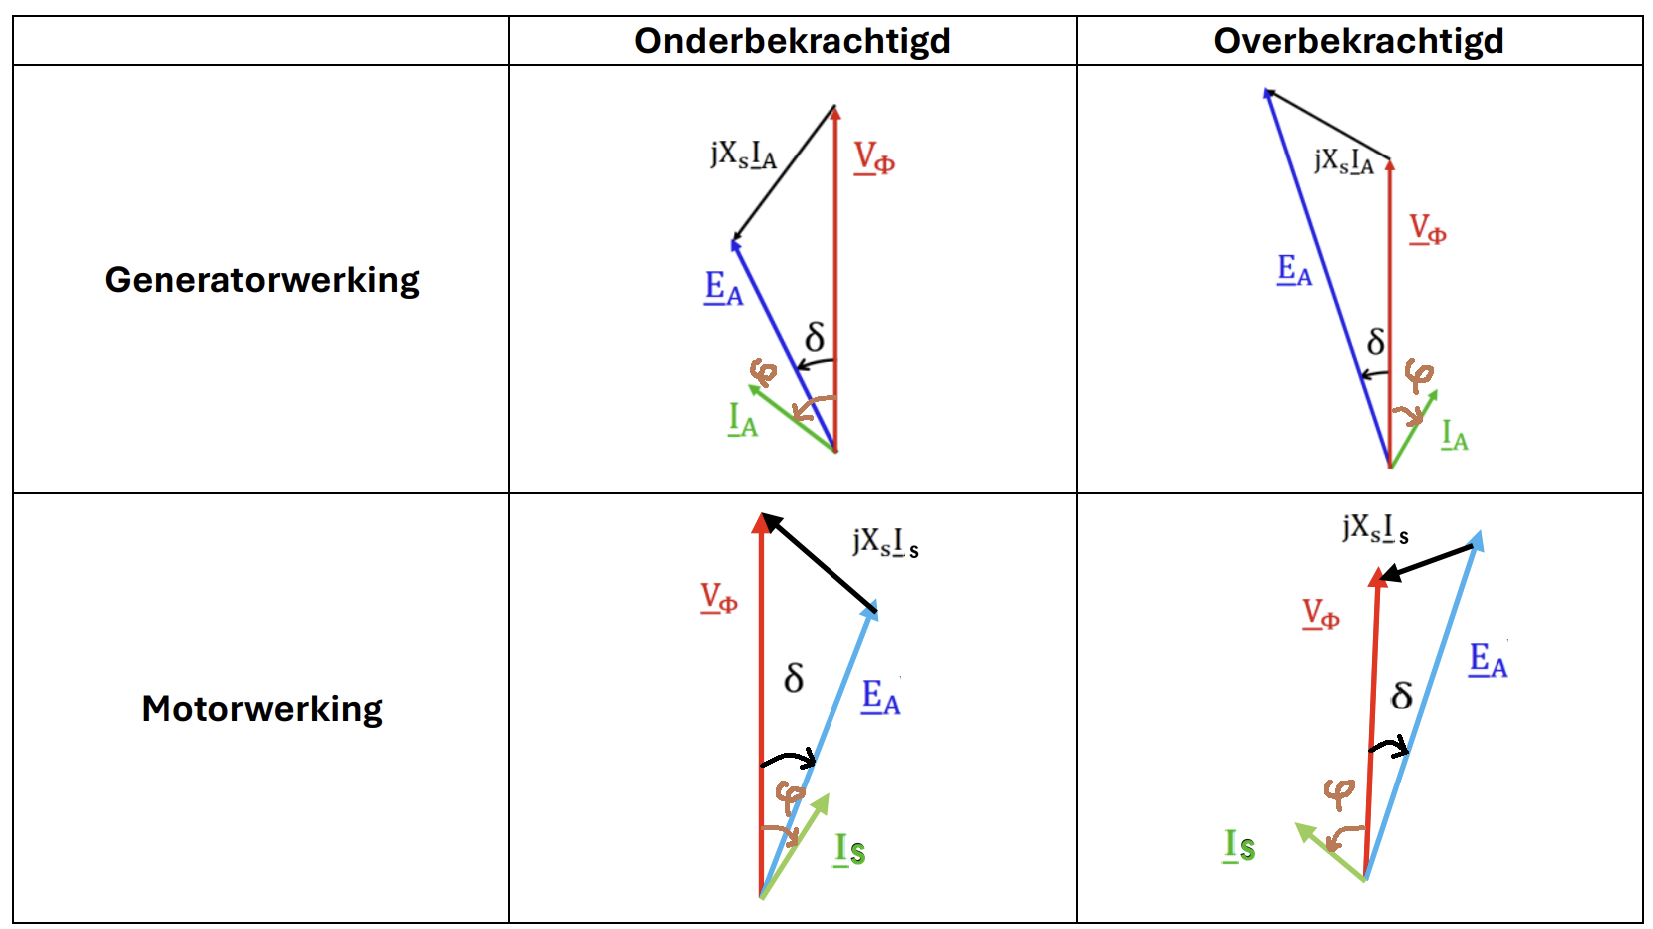
\includegraphics[width=0.8\textwidth]{assets/fasediragmamee.png}
  \caption{Fasediagrammen motor en generator, onder en overbekrachtigd}
  \label{fig:fasediragmamee.png}
 \end{figure}

Wat wel belangrijk is om op te merken is dat bij motorwerking we niet meer met $I_A$
werken maar met $I_S$ (de statorstroom, want de machine neemt nu stroom op), en wat nog
belangrijker is, is dat deze het \textbf{tegenovergestelde} is van $I_A$ dus
$I_A = - I_S$!
En dus voor de motor geldt:
\begin{align*}
    \underline{V}_{\phi} = \underline{E}_A + j \cdot X_S \cdot \underline{I}_S
\end{align*}

\subsection{Onderbekrachtiging}
Bij onderbekrachtiging is het rotorveld ($I_f$) te zwak, hierdoor is er te weinig flux in
de machine en gaat de stator dit moeten compenseren door een hogere stroom te trekken, dit
zorgt voor meer veld ($\vv{B}_{Stat}$) want als de flux daalt, daalt de inwendige spanning
$E_A$ en stijgt dus de statorstroom $I_S$.
Bij een motor wordt dit dus inductiever en bij een generator capacitiever.
Onderbekrachtigd zorgt dus dat de koppelhoek groter wordt, het kan de rotor meesleuren
maar het loopt meer achter.

\subsection{Overbekrachtiging}
Bij overbekrachtiging is het rotorveld ($I_f$) te sterk, hierdoor is er te veel flux in de
machine en gaat de stator dit moeten tegenwerken door een lagere stroom te trekken, de
stator voert dus eigelijk magnetisch veld af (levert dus reactief vermogen) wat het bij de
motor capacitiever maakt en bij de generator inductiever.
De stator wilt de rotor eigelijk afremmen waardoor de koppelhoek kleiner wordt.

\section{Vermogen en koppel}
Voor het bepalen van het vermogen van de synchrone machine gaan we van uit van een ideale
machine waarbij dus geldt dat het elektrisch vermogen gelijk is aan het mechanisch
vermogen, dus een rendement van 100.
Ook gaan we uit van een star net, dus een constante fasespanning:
\begin{align*}
    P_{elektrisch} = P_{mechanisch}
\end{align*}
Het elektrisch vermogen kunnen we schrijven als:
\begin{align*}
    \sqrt{3} \cdot U_L \cdot I_L \cdot \cos(\varphi) = 3 \cdot \underbrace{V_{\phi}}_{\text{Constant!}} \cdot I_A \cdot \cos(\varphi)
\end{align*}
Met het fasordiagram (simpele geometrie dat het stukje $I_A \cdot \cos(\varphi)$ verandert
door $\frac{\sin(\delta) \cdot E_A}{X_S}$) kunnen we dit ook schrijven als:
\begin{align*}
    P_{elektrisch} = P_{mechanisch} = P = 3 \cdot \frac{V_{\phi} \cdot E_A}{X_S} \cdot \sin(\delta)
\end{align*}
Dit is dus de formule voor het vermogen bij een ideale machine, dit is een sinusvormige
functie.
Het koppel kan dus ook bepaald worden met de formule $P = T \cdot \omega$.

\subsection{Synchronisatieverliezen}
Dat sinusvormige vermogen is dus afhankelijk van de koppelhoek $\delta$ en is maximaal op
$\delta = 90^\circ$, hierna daalt dit vermogen terug.
We willen dus eigelijk rond die 90 graden werken maar we doen het in de praktijk niet door
synchronisatieverliezen.
Bij synchronisatieverlies gaan we over de maximale koppel gaan, waardoor we niet genoeg
vermogen meer gaan hebben waardoor we eigenlijk niet meer synchroon gaan draaien, we lopen
eigelijk achter en onze hoek wordt dus groter, dit kan zo uitlopen tot we uiteindelijk een
volledige toer achter zitten.
Toeren kunnen we terugwinnen door de snelheid op te trekken, er is dus acceleratie nodig.
Daarom werken we rond een gebied van $20^\circ-30^\circ$.

\begin{figure}[H]
  \centering
  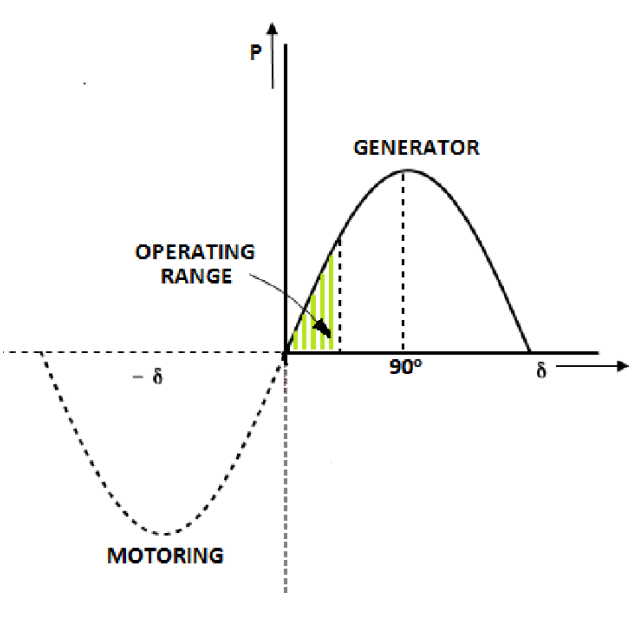
\includegraphics[width=0.5\textwidth]{assets/werkingsgebiedvoorsynchronisatieverliesµ.png}
  \caption{Vermogen ifv koppelhoek, met aanduiding van het werkingsgebied voor
  synchronisatieverlies}
  \label{fig:werkingsgebiedvoorsynchronisatieverliesµ.png}
 \end{figure}

Een plotse verandering van last (lasthoek wordt even heel groot want de rotor vertraagt
even) kan wel zorgen voor een transiënte snelheid verandering, deze gaat uiteindelijk wel
naar zijn oorspronglijke synchrone snelheid (steady-state).
Maar een te grote verandering van last kan dus toeren doen missen of de motor doen
stilvallen.

\begin{figure}[H]
  \centering
  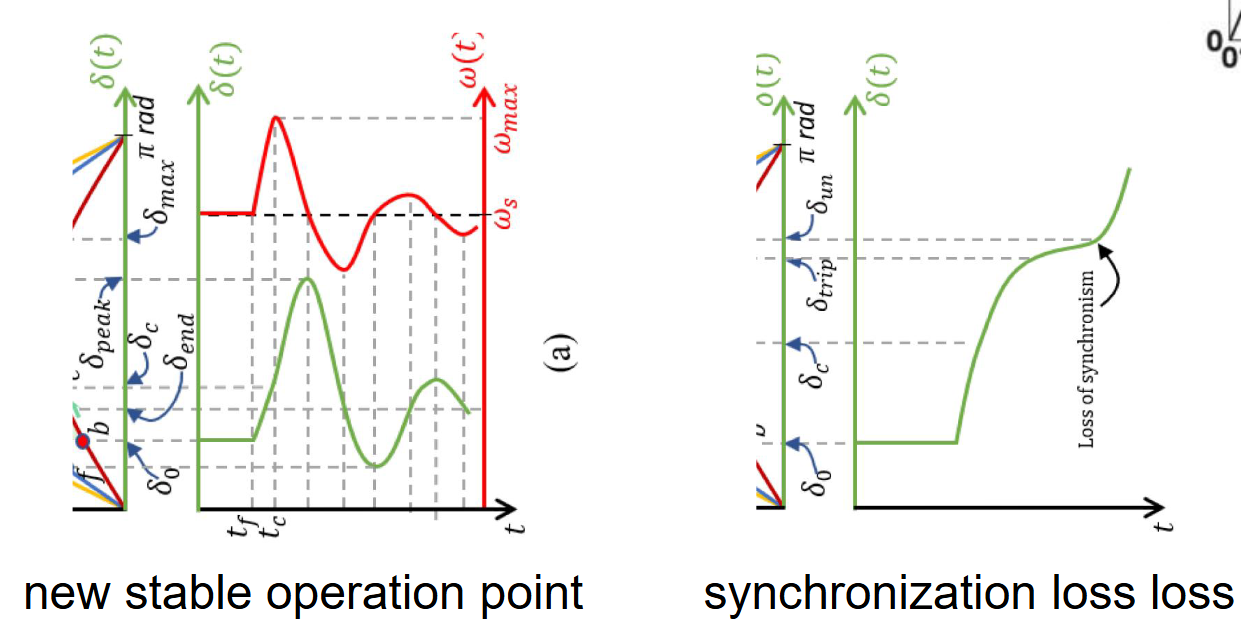
\includegraphics[width=0.6\textwidth]{assets/transienteensynchronisatieverlies.png}
  \caption{Linkse plot terug naar stabiele toestand, rechtse plot naar
  synchronisatieverlies}
  \label{fig:transienteensynchronisatieverlies.png}
 \end{figure}

\subsection{Verschil in rotorconstructie}
Als je bij een glade rotor geen stroom hebt in de rotor maar wel in stator dan gaat je
draaiveld geen invloed hebben op de rotor, er is dus geen koppel.
Bij een rotor met polen ga je wel een koppel hebben, dit is omdat het ijzer van die polen
eigelijk wilt alligneren met dat magnetisch draaiveld, ze nemen het pad van minste
\textbf{reluctantie}.
Dit noemt dus een reluctantiekoppel en heeft dus een reluctantievermogen.
Dit draagt bij aan het totaal vermogen:

\begin{figure}[H]
  \centering
  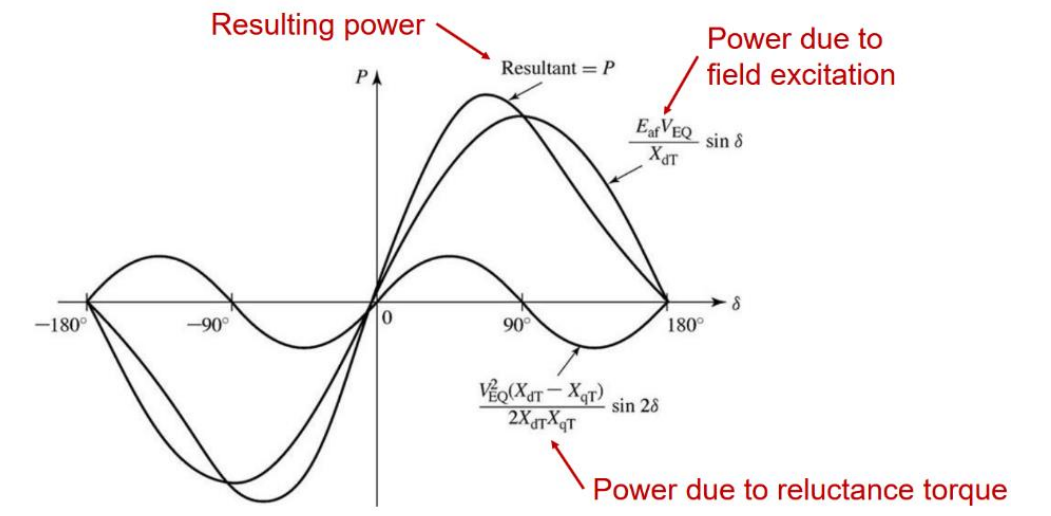
\includegraphics[width=0.6\textwidth]{assets/invloedrelucatnievermoge.png}
  \caption{Invloed reluctantievermogen}
  \label{fig:invloedrelucatnievermoge.png}
 \end{figure}

Dit reluctantievermogen piekt op een hoek van $45^\circ$ en is dus veroorzaakt door de
vorm van de rotor.

\section{Synchrone Generator}

\subsection{Eilandbedrijf}
Een synchrone generator kan in eilandbedrijf werken, dit wil zeggen dat hij niet verbonden
is met een groot net maar dat hij zelf een net vormt.
(Stand-alone).
Bvb een windturbine die een huis van stroom voorziet (lijkt mij straf ma dit is een
voorbeeld).
We gaan nu eens kijken wat er gebeurt als de belasting hierop varieert, want deze doet de
grootte van $I_A$ veranderen.

\begin{figure}[H]
  \centering
  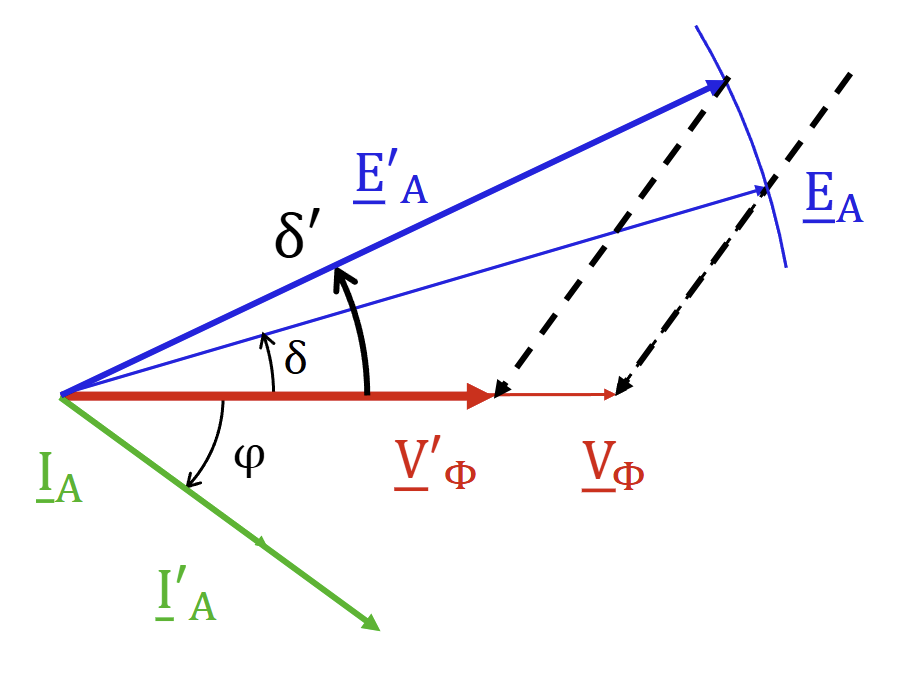
\includegraphics[width=0.5\textwidth]{assets/varierendebelastinggeneratoreilandbedrijf.png}
  \caption{Fasediagrammen bij variërende belasting van een synchrone generator in
  eilandbedrijf}
  \label{fig:varierendebelastinggeneratoreilandbedrijf.png}
 \end{figure}

We weten dat meer belasting zorgt voor een grotere lasthoek, en aangezien $E_A$
afhankelijk is van de bekrachtiging $I_f$ blijft deze constant, je ziet dat daardoor
$V_{\phi}$ kleiner is geworden en de stroom groter.
Als we $V_{\phi}$ groter willen zullen we met de bekrachtiging moeten spelen om $E_A$
groter te maken.

\subsection{Meerdere (Parallelle) generatoren}
Je kan ook meerdere generatoren in parallel zetten, dit heeft als voordelen dat dit meer
betrouwbaar is want als één uitvalt werkt de rest wel nog, veel generatoren zorgen ook
voor een stabieler net.
Condities die nodig zijn voor het parallel schakelen zijn de volgende:

\begin{itemize}
    \item Ze moeten dezelfde spanning hebben
    \item Ze moeten dezelfde frequentie hebben
    \item Ze moeten dezelfde fasehoek hebben
    \item Ze moeten dezelfde fasevolgorde (fase sequentie) hebben
\end{itemize}

Ze moeten niet percee de zelfde snelheid of zelfde poolpaartal hebben (behalve als ze op
de zelfde as zitten)

\begin{conceptbox}[Star net]
    Een star net is een net waarvan de spanning constant is, hier zijn een groot aantal
    generatoren parallel geschakeld.
    Ze hebben een systeem operator (zoals Elia)
\end{conceptbox}

\subsection{Rating van een synchrone generator}
Nu gaan we kijken naar de limieten van de synchrone machine, dit is belangrijk want we
willen weten wat de maximale belasting is die we kunnen leveren.
We hebben hiervoor een aantal limieten.

\begin{figure}[H]
  \centering
  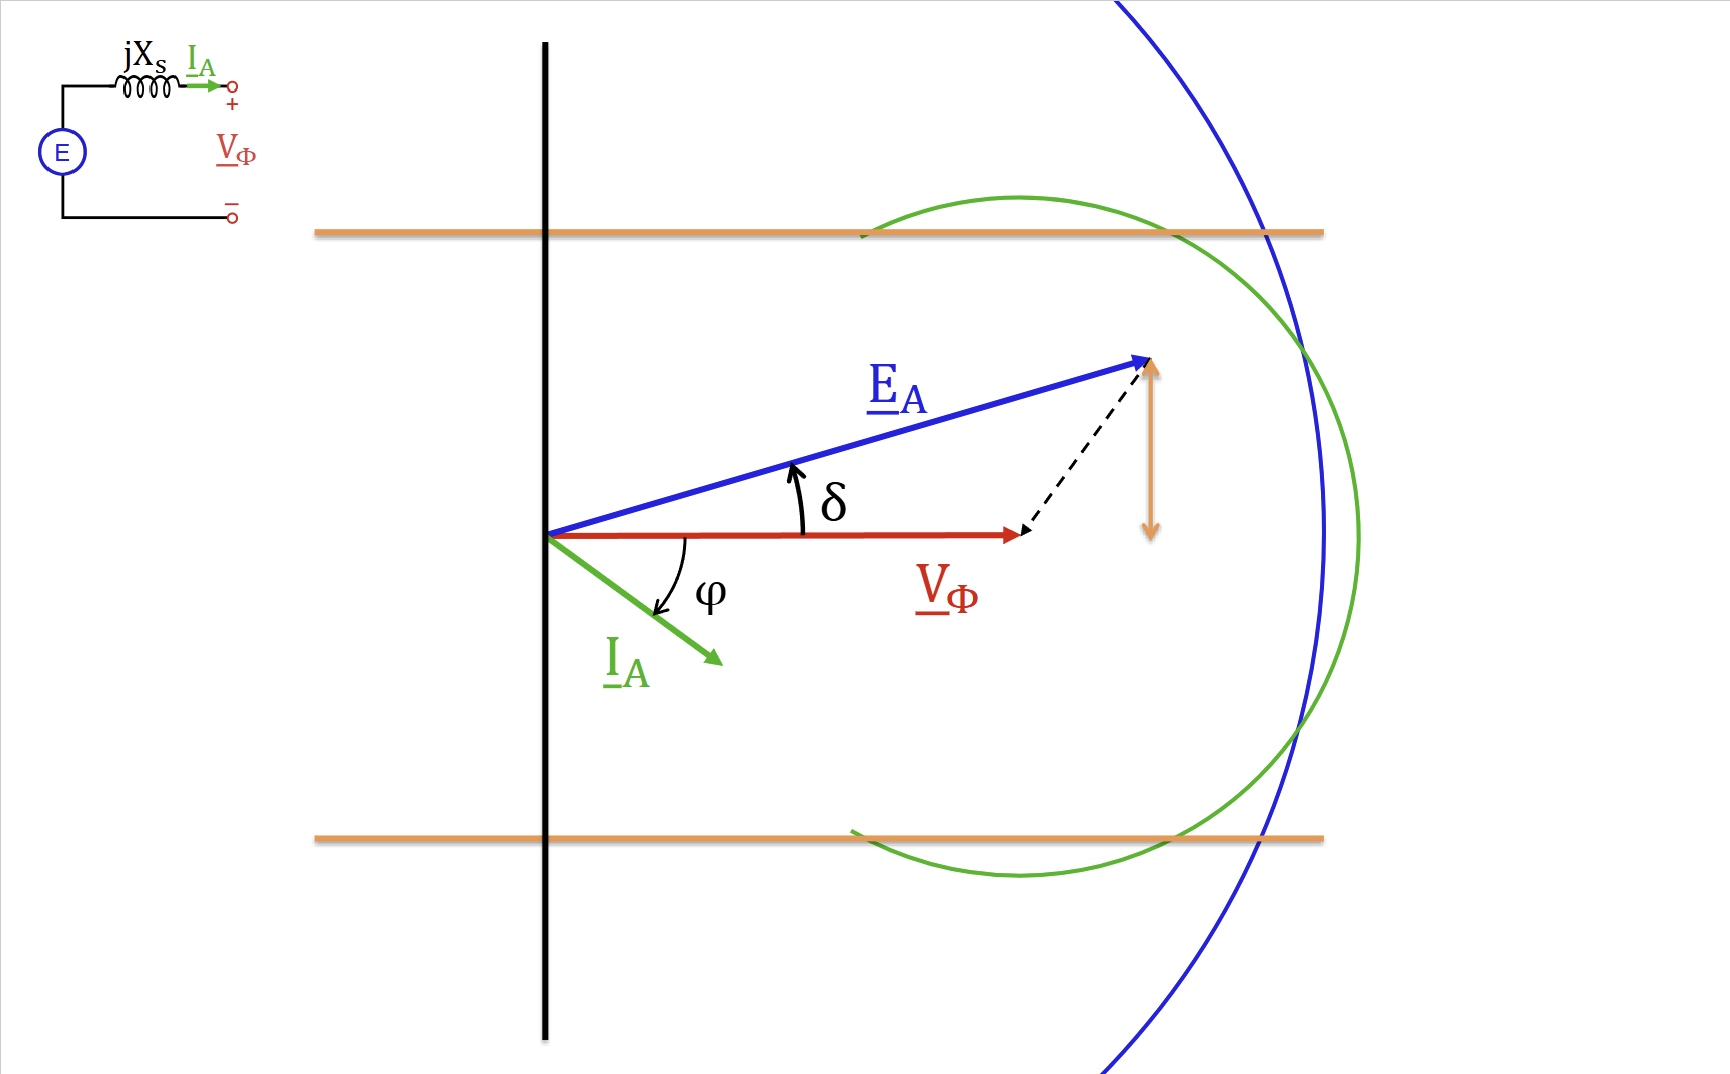
\includegraphics[width=0.7\textwidth]{assets/limietensynchronemachine.png}
  \caption{Ratings van een synchrone machine}
  \label{fig:limietensynchronemachine.png}
 \end{figure}

We hebben een vermogen grens (oranje lijnen) en thermische grenzen (groen en blauwe
lijnen).
Ook moet natuurlijk nog de lasthoek onder die 90 graden blijven.
We beginnen met dit fasediagram waar de fasespanning constant is (star net).
Dit fasediagram is trouwens voor 1 van de 3 fases van deze machine getekend, de andere 2
zijn met 120 graden verschoven.

$I_A$ mag niet te groot zijn want anders heb je overhitting, deze grens is getekent rond
het punt waar de fasespanning daar eindigt want daar begint het gedeelte
$j \cdot X_S \cdot I_A$ en dan wordt $X_S$ gewoon geschaald.
(Om voor beide gevallen van $j \cdot X_S \cdot I_A$ en $j \cdot X_S \cdot I_S$ te kunnen
werken, wordt dit vaak ook $\Delta u$ genoemd)

Hetzelfde voor $I_f$, maar hier dan met een grens voor $E_A$ aangeduid omdat dit evenredig
is.

Er is ook een mechanisch vermogen van de as, dus hoeveel je motor aankan, dit is
weergegeven met de oranje horizontale lijnen.
De pijl van $E_A$ mag hier niet boven of onder.
Meestal is dit de eerste limiet die je bereikt.

De zwarte verticale lijn toont tot waar de lasthoek mag gaan.
Eigelijk heb je pas vanaf 180 graden dat die toeren overslaat maar voorbij 90 graden loop
je het risico voor asynchroonwerking.

\section{Synchrone Motor}

\subsection{Motorwerking}
Nu kijken we naar de motorwerking, we gaan hier uit van een gladde rotor alsook dat de
rotor even snel draait als het draaiveld van de stator ($\omega_s$) wat in het echt wel
moeilijk is.
Even kleine herhaling maar we weten hierbij dus dat de lasthoek negatief is, dus
tegengesteld aan de draaizin.
Er wordt hier een koppel opgewekt met de volgende formule:
\begin{align*}
    T = k \cdot B_{mut} \cdot B_R \cdot \sin(\delta)
\end{align*}
Bij het equivalent schema gebruiken we nu ook de motorreferentie:

\begin{figure}[H]
  \centering
  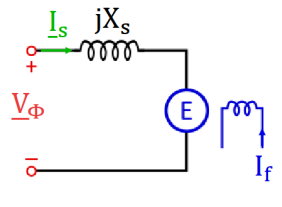
\includegraphics[width=0.3\textwidth]{assets/equivschemamotorref.png}
  \caption{Equivalent schema van een synchrone machine met motorreferentie}
  \label{fig:equivschemamotorref.png}
 \end{figure}

Hierbij mogen we ook niet vergeten dat onze vergelijking nu deze is:
\begin{align*}
    \underline{V}_{\phi} = \underline{E}_A + j \cdot X_S \cdot \underline{I}_S
\end{align*}
Onze stroom $I_S$ loopt nu IN de machine, dus $\Delta u$ heeft een ander teken.
Het wordt dus opgeteld bij $E_A$, wat ook zichtbaar is op het fasediagram:

\begin{figure}[H]
  \centering
  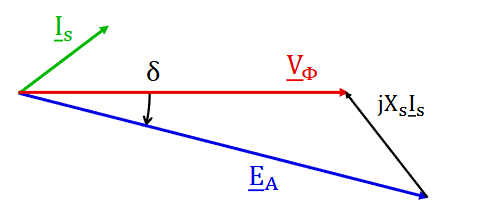
\includegraphics[width=0.5\textwidth]{assets/motorwerkingfasediagram.png}
  \caption{Fasediagram Overbekrachtigde Motor}
  \label{fig:motorwerkingfasediagram.png}
 \end{figure}

We zien hier dus ook dat de stroom $I_S$ loodrecht staat op $\Delta u$ (wat altijd is, ik
had het gewoon nog niet eerder gezegd) en ook dat het na ijlt op $\Delta u$ (dit zie je
duidelijker als je de aangrijppunten samenneemt, dit is ook altijd)

\subsection{Karakteristieken}

\subsubsection{Koppel-toerentalkarakteristiek}
Het koppel-toerentalkarakteristiek van een synchrone motor ziet er zo uit (met de
veronderstelling van een star net!):

\begin{figure}[H]
  \centering
  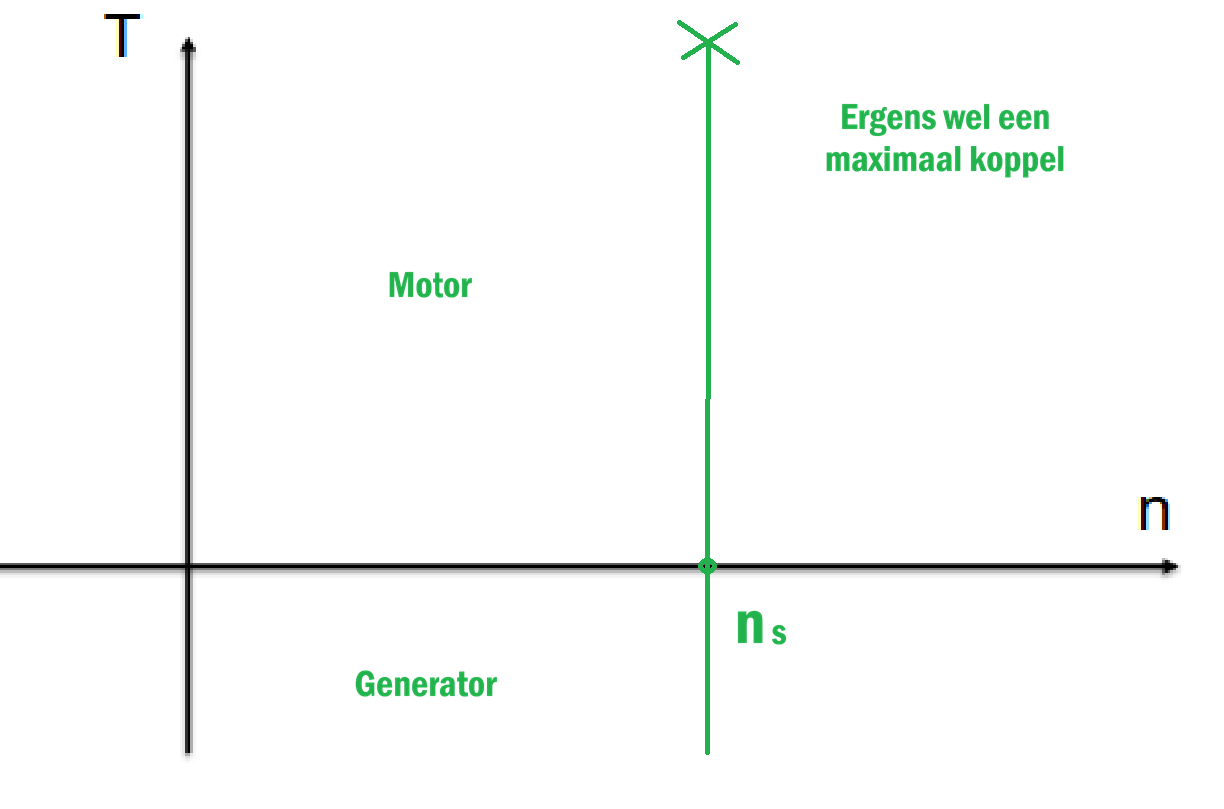
\includegraphics[width=0.5\textwidth]{assets/TNsynchronempotor.png}
  \caption{Koppel-toerentalkarakteristiek van een synchrone motor}
  \label{fig:TNsynchronempotor.png}
 \end{figure}

We zien dat dit gewoon een rechte is op een constante snelheid $n_s$, dit is de ideale
machine dus.
Het kan in principe onder de n-as gaan want je kan in generator werking zitten.
Het grote nadeel hier is dus dat de motor niet zelfstartend is.

\subsubsection{Belastingsvariatie}
Wat gaat de synchrone motor nu doen als de belasting verandert?
We nemen hier dus ook star net aan alsook dat de excitatie vast staat (dus gelijke $E_A$).
Dus $\omega_s$ constant.
Zoals we eerder zagen gaat de afstand tussen $V_{\phi}$ en $E_A$ groter worden als we meer
belasten, de lasthoek veranderd dus, dit effect plotten we op de T-$\delta$
karakteristiek.

\begin{figure}[H]
  \centering
  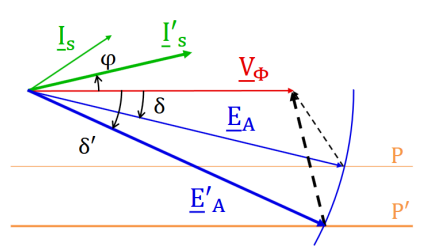
\includegraphics[width=0.5\textwidth]{assets/fasediagrambelastingsvariatiemotor.png}
  \caption{Fasediagram bij belastingsvariatie van een synchrone motor}
  \label{fig:fasediagrambelastingsvariatiemotor.png}
 \end{figure}

We zien dat $\delta$ groter wordt, $\Delta u$ veranderd en dus ook $I_S$ want deze moet
loodrecht hierop staan.
De stroom wordt hier dus minder capacitief en de grootte veranderd ook wat.

\subsubsection{Koppel-lasthoekkarakteristiek}
Dus de belastingvariatie varieert de lasthoek ook, hier is het bij een motor dus wordt het
effect van de lasthoek op het koppel weergegeven met de volgende formule:
\begin{align*}
    T = \frac{3}{\omega_s} \cdot \frac{V_\phi \cdot E}{X_S} \cdot \sin(-\delta_{load})
\end{align*}
Ook weergegeven met deze grafiek:

\begin{figure}[H]
  \centering
  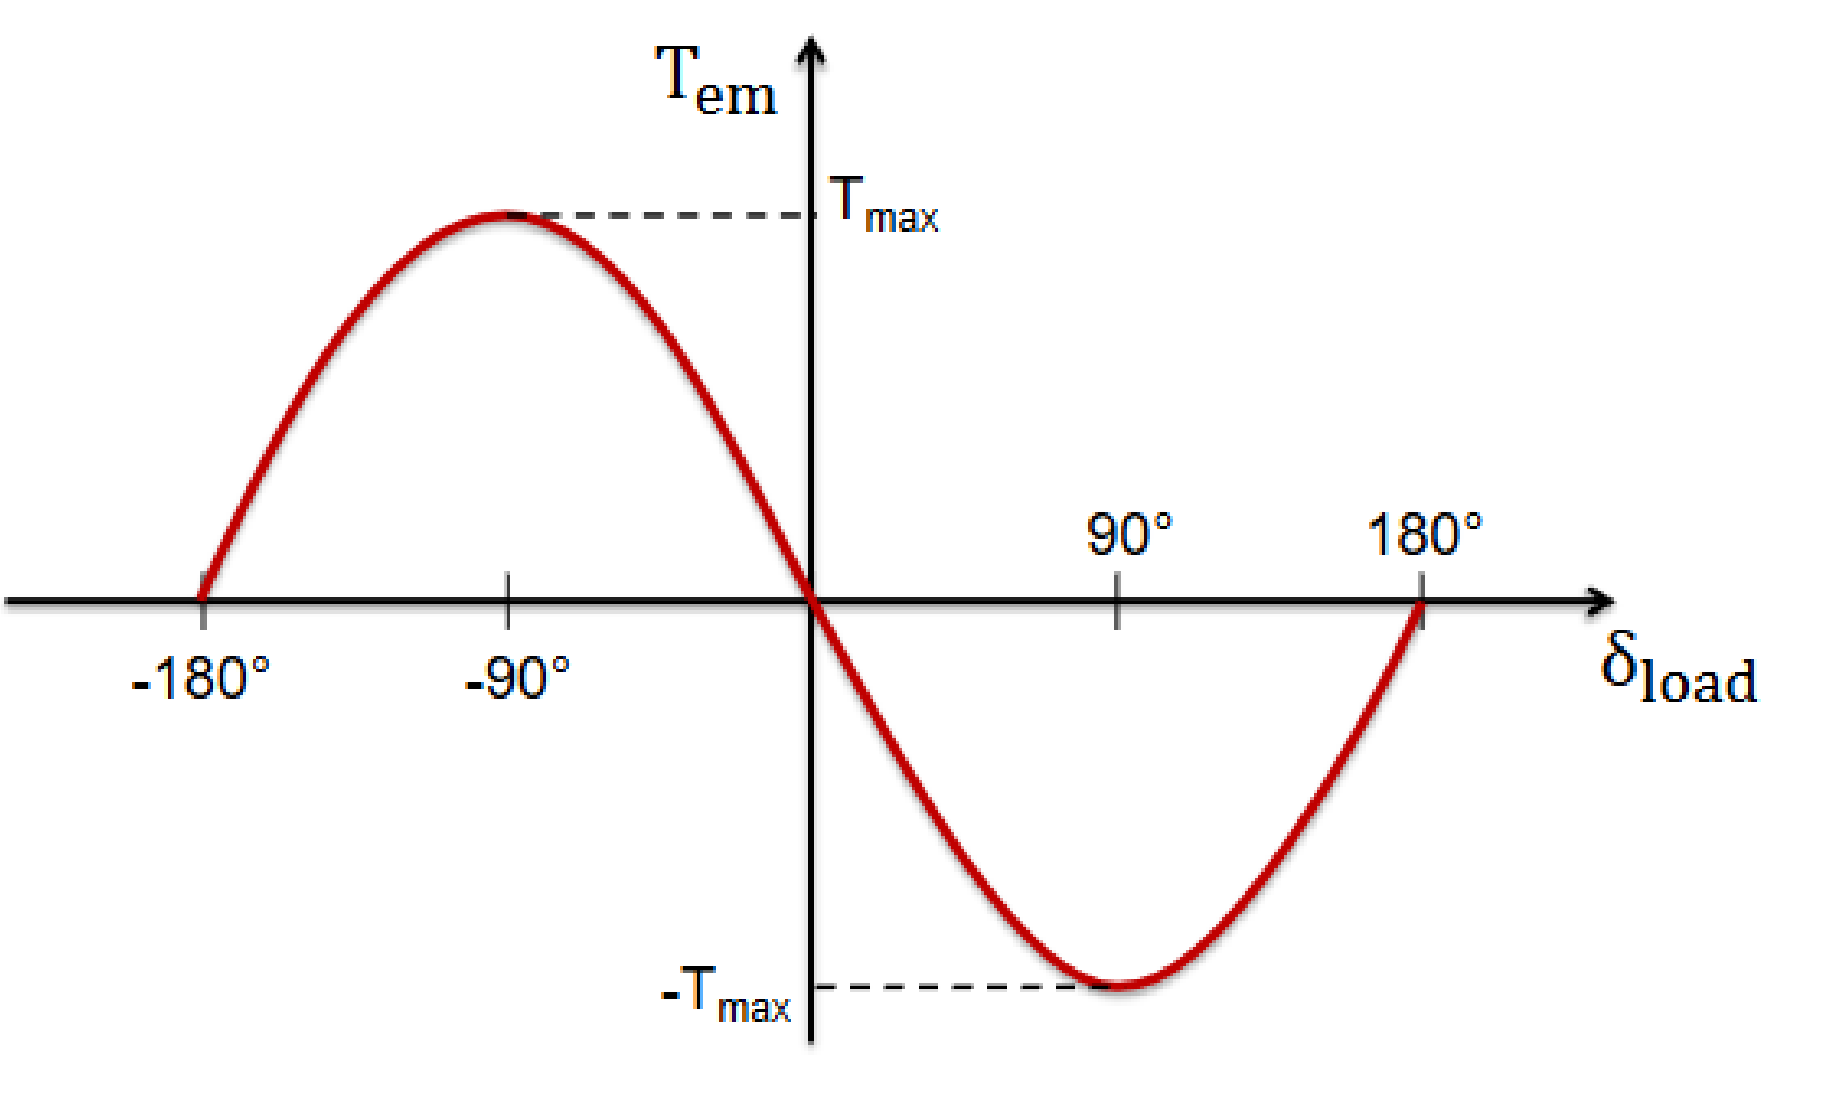
\includegraphics[width=0.5\textwidth]{assets/koppellastkarakteristiekmotor.png}
  \caption{Koppel-lasthoekkarakteristiek van een synchrone motor}
  \label{fig:koppellastkarakteristiekmotor.png}
 \end{figure}

De sinus golf links is voor een motor, die dat de negatieve koppel heeft rechts is voor
generator (daar is de lasthoek dus ook groter dan 0).

\subsubsection{Effect van spanningsdip op het koppel}
Dan gaan we nu eens kijken wat er gebeurd als je een plotse spanningsdaling krijg aan de
klemspanning (van meer dan 10\%).
Via de formule weten we dat het koppel dan zal dalen, waardoor de kans op
synchronisatieverlies toeneemt

\begin{figure}[H]
  \centering
  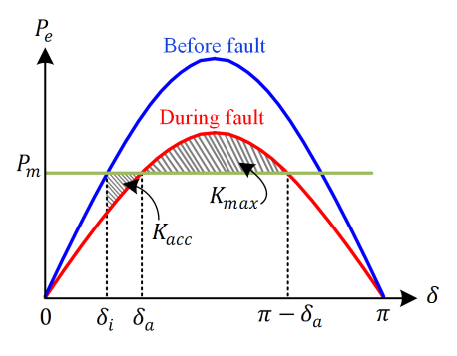
\includegraphics[width=0.5\textwidth]{assets/effectspanningsdip.png}
  \caption{Effect van spanningsdip op het koppel}
  \label{fig:effectspanningsdip.png}
 \end{figure}

In de figuur hierboven zien we dit effect van die spanningsdip, het is hier wel met
vermogen weergegeven ma das zo goed als het zelfde want dat is afhankelijk van koppel.
We zien de groene lijn, dit is de last die je motor draagt.
Er is daar helemaal links een snijpunt met de blauwe curve, dat is je oorspronkelijk
werkingspunt.
Als er een spanningsdip voorkomt wordt het eigelijk die rode curve, je werkingspunt
verschuift dan eigelijk wat waardoor je lasthoek vooral gaat slingeren (en je snelheid
ook) zoals een transiënte.
Uiteindelijk wordt dan een nieuw werkingspunt gevonden, en dit nieuwe werkingspunt is
stabiel als die oppervlakte van $A_1$ kleiner is als die van $A_2$, anders heb je te
weinig vermogen en worden toeren gemist en krijg je dus synchronisatie verlies.

\begin{figure}[H]
  \centering
  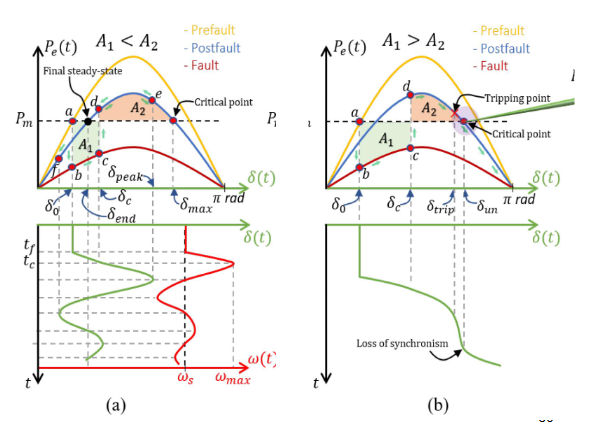
\includegraphics[width=0.5\textwidth]{assets/transienetespannignsdip.png}
  \caption{Transiëne effecten van spanningsdip}
  \label{fig:transienetespannignsdip.png}
 \end{figure}

\newpage

\subsubsection{Effect van excitatie variatie}
Hier gaan we zien wat er gebeurd als je de DC-stroom die het veld bekrachtigd (dus $I_f$)
gaat variëren.
We houden hier $V_{\phi}$ constant.
Wat we zien is dat de interne spanning ook zal stijgen in de vorm van een V-curve als je
het plot met de excitatiestroom, een mooie gif hiervan is te vinden op toledo, hier is
allesinds een screenshot daarvan:

\begin{figure}[H]
  \centering
  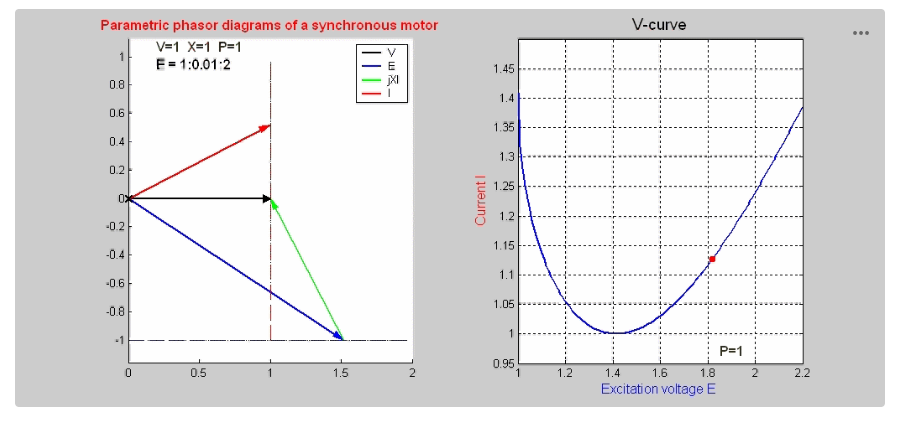
\includegraphics[width=0.6\textwidth]{assets/vcurvevarierenexcitatiestroom.png}
  \caption{V-curve bij variatie van excitatiestroom}
  \label{fig:vcurvevarierenexcitatiestroom.png}
 \end{figure}

Het grote voordeel is dat door dit te variëren je kan bepalen hoe de motor zich gaat
gedragen (resistief, inductief of capacitief), het liefst wil je capacitief want dan lever
je vermogen aan het net.
Resistief heb je trouwens op het minimum van de curve, links daarvan is inductief, rechts
daarvan is capacitief.
Ook zie je in de figuur dat dit bij een constant vermogen is, dus verschillende V-curves
zijn opgesteld voor verschillende vermogens:

\begin{figure}[H]
  \centering
  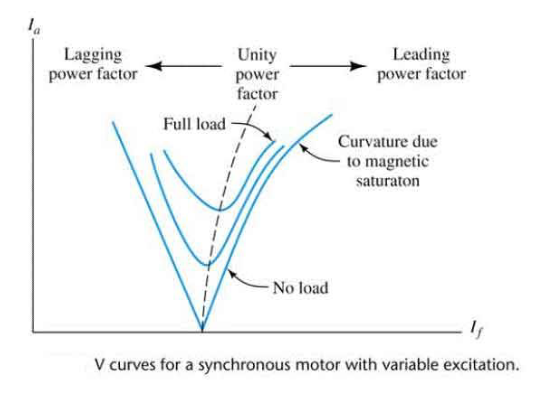
\includegraphics[width=0.5\textwidth]{assets/Vcurvesvoorverschillendevermogens.png}
  \caption{V-curves voor verschillende vermogens}
  \label{fig:Vcurvesvoorverschillendevermogens.png}
 \end{figure}

Die scherpe V-curve helemaal onderaan is de V-curve bij nullast, dit zie je want $I_a$ kan
hier 0 zijn, maar niet altijd!
Ze kunnen verschillen van nul want deze curve is bij 0 Watt, niet 0A.
Ook zien we die zwarte stippelijn een beetje afbuigen, dit is door verzadiging.

\section{Starten van de synchrone motor}
Hoe starten we nu de synchrone motor?
Want deze heeft een constante snelheid, die kan alleen draaien op $\omega_s$ terwijl in
het begin de snelheid 0 is.
Er is niet genoeg koppel dus zoasl we zien in deze T-n karakteristiek van de synchrone
machine met de nodige last:

\begin{figure}[H]
  \centering
  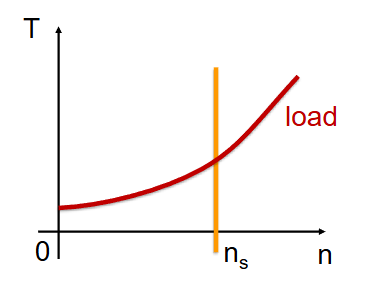
\includegraphics[width=0.3\textwidth]{assets/tnmetnodigdelast.png}
  \caption{Karakteristiek met last}
  \label{fig:tnmetnodigdelast.png}
 \end{figure}

Er zijn verschillende startmethodes die we kunnen gebruiken om de motor toch te doen
starten.

\subsection{Het reduceren van elektrische frequentie (Frequentieomvormer)}
We gebruiken een frequentieomvormer om de frequentie geleidelijk aan van 0 tot f te doen
stijgen, omdat $n_s = \frac{60f}{p}$.
Zo kan de snelheid geleidelijk stijgen.
{\color{red}MAAR!}:

De spanning E is ook afhankelijk van f met:
\begin{align*}
 E =  \sqrt{2}\cdot \pi \cdot N_c \cdot \phi \cdot f = K \cdot \phi \cdot \omega
\end{align*}
Dus we gaan moeten zien dat als we de frequentie verhogen, we de spanning E ook verhogen,
anders is de stroom $I_s$ te groot ($V_{\phi} = E + j \cdot X_S \cdot I_S$), ook gaat het
koppel wat lager moeten worden want
$T = - \frac{3}{\omega_s} \cdot \frac{V_\phi \cdot E}{X_S} \cdot \sin(\delta)$, dus als
$\omega_s$ stijgt, daalt T.
Dit is dus een nadeel van deze methode.

\subsection{Hulpmotor gebruiken}
Bij het opstarten met behulp van een hulpmotor gaan we eigenlijk een externe motor
gebruiken,
zoals een asynchrone motor die wel kan opstarten vanaf stilstand.
Deze gaat dan de synchrone
motor aandraaien, waardoor deze ook gestart geraakt.
We gaan dan eigenlijk eerst de motor opstarten als een generator, waardoor we de motor
kunnen afstemmen op het net, waardoor we de frequentie, spanning en fasehoek juist kunnen
instellen. Hierdoor kunnen we grotere vermogens starten.

\subsection{Damper/Amortisseur windingen gebruiken (Demperkooi)}
Om de synchrone machine te kunnen doen aanlopen, kunnen we ook gebruik maken van een
damperwikkeling.
Dit is eigenlijk zoals een squirrel cage rotor en gelijkaardig aan de inductiemachine:
het zijn kortgesloten koperen staven in de rotor, verbonden door platen.
Bij stilstand beweegt het draaiveld relatief ten opzichte van de staven, wat een stroom in
de staven induceert die kunnen lopen doordat ze kortgesloten zijn.
Samen met het veld wordt hierdoor een kracht uitgeoefend op de staven, die de snelheid van
de rotor optrekt zonder dat daar DC-bekrachtiging voor nodig is.
Zodra de rotor op synchrone snelheid zit, is er geen relatieve beweging meer, dus ook geen
extra geïnduceerde stroom en dus geen verliezen daaraan, de wikkeling ligt dan relatief
stil.

\begin{figure}[H]
  \centering
  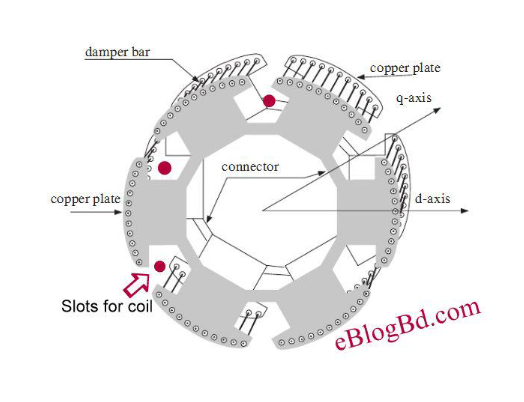
\includegraphics[width=0.5\textwidth]{assets/demperwikkelinge.png}
  \caption{Demperwikkeling in een synchrone machine}
  \label{fig:demperwikkelinge.png}
 \end{figure}

\section{Oefeningen synchrone machines}

\begin{oefenblok}[Oefening 4.6 van Slides]
\textbf{Opgave:}
\newline
The internal generated voltage $E_A$ of a 2-pole, $\Delta$-connected, 60 Hz, three phase
synchronous generator is 14.4 kV, and the terminal voltage $V_T$ is 12.8 kV.
The synchronous reactance of this machine is 4 $\Omega$, and the armature resistance can
be ignored.
\begin{itemize}
 \item a) If the torque angle of the generator $\delta$ is $18^\circ$, how much power is
 being supplied by this generator at the current time?
 \item b) What is the power factor of the generator at this time?
 \item c) Sketch the phasor diagram under these circumstances.
 \item d) Ignoring losses in this generator, what torque must be applied to its shaft by
 the prime mover at these conditions?
\end{itemize}
\textbf{Oplossing:}
\newline
We schrijven eerst rap onze gegevens op:
\begin{itemize}
    \item $p = 1$
    \item $f = 60 Hz$
    \item $E_A = 14.4 kV$
    \item $V_T = V_\phi = 12.8 kV$
    \item $X_S = 4 \Omega$
    \item $\delta = 18^\circ$
\end{itemize}
\textbf{a)}
We werken in generatorreferentie dus voor het vermogen gebruiken we de volgende formule
($V_T = V_\phi$ want het is een $\Delta$-verbinding):
\begin{align*}
    P = 3 \cdot \frac{V_\phi \cdot E_A}{X_S} \cdot \sin(\delta) = 3 \cdot \frac{12.8 kV \cdot 14.4 kV}{4 \Omega} \cdot \sin(18^\circ) = 42.7 MW
\end{align*}
\textbf{b)}
Het vermogen dat we net hadden berekend was het elektrisch vermogen, dit kunnen we ook
berekenen met de formule:
\begin{align*}
    P = 3 \cdot V_\phi \cdot I_A \cdot \cos(\varphi)
\end{align*}
$I_A$ kunnen we berekenen met de formule:
\begin{align*}
    \underline{V}_{\phi} = \underline{E}_A - j \cdot X_S \cdot \underline{I}_A \\
    \rightarrow j \cdot X_S \cdot \underline{I}_A = \underline{E}_A - \underline{V}_{\phi} \\
    \rightarrow \underline{I}_A = \frac{\underline{E}_A - \underline{V}_{\phi}}{j \cdot X_S}
\end{align*}
Dit kan je invullen in je rekenmachine of grafisch met een fasediagram vinden zodat je
krijgt dat:
\begin{align*}
    I_A = \frac{14.4 kV \angle 18^\circ - 12.8 kV \angle 0^\circ}{j \cdot 4 \Omega} = 1.13 kA \angle -11.37^\circ
\end{align*}
En dus de arbeidsfactor gelijk is aan:
\begin{align*}
    \cos(\varphi) = \cos(-11.37^\circ) = 0.981
\end{align*}
\textbf{c)}
Nu simpelweg al deze vectoren tekenen, niet vergeten dat $I_A$ loodrecht staat op
$j \cdot X_S \cdot I_A$ en dat $V_\phi = E_A - j \cdot X_S \cdot I_A$.
\begin{figure}[H]
  \centering
  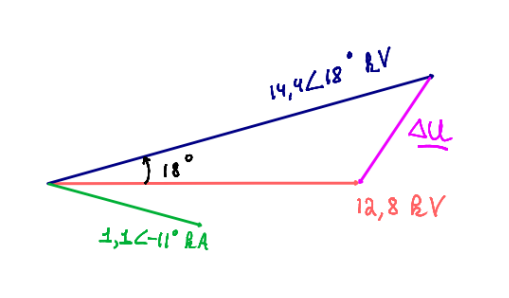
\includegraphics[width=0.5\textwidth]{assets/fasediagramoefening.png}
  \caption{Fasediagram van oefening 4.6}
  \label{fig:fasediagramoefening.png}
 \end{figure}
\textbf{d)}
We mogen verliezen negeren dus geldt dat $P_{elektrisch} = P_{mechanisch}$, dus het koppel
dat de as moet leveren is:
\begin{align*}
    P_m = P_{el} = T \cdot \omega_s 
\end{align*}
\begin{align*}
    \rightarrow T = \frac{P_m}{\omega_s} = \frac{42.7 MW}{2 \cdot \pi \cdot 60 Hz} = 113.2 kNm
\end{align*}
\end{oefenblok}

\begin{oefenblok}[Oefening 7.19 van Slides]
\textbf{Opgave:}
\newline
A four-pole, 25 kW, 250 V separately excited DC motor is
mechanically coupled to a threephase four-pole, 25 kVA, 460 V,
cylindrical pole synchronous generator. The DC motor is connected
to a constant 250 V DC supply and the ac generator is connected to
a 460 V fixed voltage, fixed frequency, threephase grid. The
synchronous reactance of the synchronous generator is 6.6 $\Omega$. The
armature resistance of the DC motor is 22 m$\Omega$. All unspecified
losses are to be neglected.
\begin{itemize}
 \item a) If the two machines act as a motor-generator set receiving power from the
DC source and delivering power to the ac grid, what is the internal phase
voltage $E_{SM}$ of the ac machine when it delivers 25kW at unity power factor?
What is the internal voltage (back-emf) of the DC motor?
 \item b) Leaving the field current of the ac machine at the value corresponding to the
condition of part (a), what adjustment can be made to reduce the power
transfer between the two machines to zero? Under this condition of zero
power transfer, what is the armature current of the DC machine? What is
the armature current of the ac machine?
 \item c) Leaving the field current of the ac machine as in parts (a) and (b), what
adjustment can be made to cause the transfer of 25kW from the ac source
to the DC source? Under these conditions, what are the armature current
and internal voltage of the DC machine? What will be the magnitude and
phase of the current in the ac machine? 
\end{itemize}
\textbf{Oplossing:}
\dots ({\color{red}Nog niet aan begonnen})
\end{oefenblok}

\begin{oefenblok}[Oefening 5-3 van Slides]
\textbf{Opgave:}
\newline
A 230-V, 50 Hz, two-pole synchronous motor draws 40 A from the line at unity power factor
and full load.
Assuming that the motor is lossless, answer the following questions:
\begin{itemize}
 \item a) What is the output torque of this motor? Express the answer in newton-meters.
 \item b) What must be done to change the power factor to 0.85 leading?
 Explain your answer, using phasor diagrams.
 \item c) What will the magnitude of the line current be if the power factor is adjusted
 to 0.85 leading?
\end{itemize}
\textbf{Oplossing:}
\dots ({\color{red}Nog niet aan begonnen})
\end{oefenblok}

\begin{oefenblok}[Oefening 5-10 van Slides]
\textbf{Opgave:}
\newline
A synchronous machine has a synchronous reactance of 1.0 $\Omega$ per phase and an
armature resistance of 0.1 $\Omega$ per phase.
If $E_A = 460 \angle -10^\circ$ V and $V_\phi = 480 \angle 0^\circ$ V, is this machine a
motor or a generator?
How much power $P$ is this machine consuming from or supplying to the electrical system?
How much reactive power $Q$ is this machine consuming from or supplying to the electrical
system?
\newline
\textbf{Oplossing:}
\dots ({\color{red}Nog niet aan begonnen})
\end{oefenblok}

\begin{oefenblok}[Oefening 5-17 van Slides]
\textbf{Opgave:}
\newline
A 440-V, 60-Hz, three-phase, Y-connected synchronous motor has a synchronous reactance of
1.5 $\Omega$ per phase.
The field current has been adjusted so that the torque angle $\delta$ is $25^\circ$ when
the power supplied by the generator is 80 kW.
\begin{itemize}
 \item a) What is the magnitude of the internal generated voltage $E_A$ in this machine?
 \item b) What are the magnitude and angle of the armature current in the machine?
 What is the motor's power factor?
 \item c) If the field current remains constant, what is the absolute maximum power this
 motor could supply?
\end{itemize}
\textbf{Oplossing:}
\dots ({\color{red}Nog niet aan begonnen})
\end{oefenblok}

% ==================================================================

\newpage
